\documentclass[UTF8]{report}
\usepackage{graphicx}
\usepackage{xetexko}

\title{%
    <컴퓨터프로그래밍 3> 실습 보고서 \\ 
    \large [제 06 주] 성적처리}
\author{201704150 허강준}
\date{\today}


\begin{document}
    \maketitle
    \tableofcontents

    \chapter{프로그램 설명서}
        본 보고서에서는 성적 처리를 위한 객체를 정의하고 처리하는 프로그램에 대해 기술한다.

        \section{프로그램의 전체 설계 구조 (MVC 등)}
            
            \paragraph{%
                \normalfont 성적 처리 프로그램은 크게 프로그램의 제어를 담당하는 Controller인 \texttt{AppController}, 입/출력을 담당하는 View인 \texttt{AppView}, 그리고 성적 처리를 위한 모델인 \texttt{LectureClass} 로 나뉜다.
            }

            \paragraph{%
                \normalfont 이전 과제와는 달리 \texttt{AppController}를 일반 함수에서 클래스 기반의 객체로 변경하였으며 프로그램 처리를 위한 각종 멤버들(argc, argv, LectureClass 객체)을 새로 정의하였다.
            }
            
        \section{함수 설명서}

            모델 객체 관련 메서드의 경우 클래스명::메서드명 으로 기술한다. \texttt{static} 메서드의 경우 앞에 \texttt{static}을 붙인다.
            
            \paragraph{\texttt{static AppView::WriteLine(const char* str)}}
            \paragraph{%
                \normalfont 문자열을 화면에 출력한다.
            }

            \paragraph{\texttt{static AppView::out\_average(float avg)}}
            \paragraph{%
                \normalfont 성적 평균을 출력한다.
            }

            \paragraph{\texttt{static AppView::out\_aboveAvg(int count)}}
            \paragraph{%
                \normalfont 평균보다 위의 학생이 몇명인지 출력한다.
            }

            \paragraph{\texttt{static AppView::out\_max(int max)}}
            \paragraph{%
                \normalfont 최고점을 출력한다.
            }

            \paragraph{\texttt{static AppView::out\_min(int min)}}
            \paragraph{%
                \normalfont 최저점을 출력한다.
            }
            
            \paragraph{\texttt{static AppView::out\_gradeCount(int grades[5])}}
            \paragraph{%
                \normalfont 학점별 인원을 출력한다.
            }

            \paragraph{\texttt{static AppView::error\_scoreOutofRange()}}
            \paragraph{%
                \normalfont 입력된 점수가 정상 범위에서 벗어났음을 알리는 에러메세지를 출력한다.
            }

            \paragraph{\texttt{static AppView::error\_noRecordInput()}}
            \paragraph{%
                \normalfont 입력된 점수가 없음을 알리는 에러메세지를 출력한다.
            }

            \paragraph{\texttt{static AppView::out\_studentInfo(int score, char grade)}}
            \paragraph{%
                \normalfont 학생의 점수와 학점을 출력한다.
            }

            \paragraph{\texttt{static AppView::inputContinuable()}}
            \paragraph{%
                \normalfont y/n 입력을 통해 입력을 계속할 건지 질의한다.
            }

            \paragraph{\texttt{static AppView::inputScore()}}
            \paragraph{%
                \normalfont 점수를 입력받는다.
            }

            \paragraph{\texttt{static AppController::create(int argc, char* argv)}}
            \paragraph{%
                \normalfont \texttt{AppController}객체를 생성한다. \texttt{LectureClass}에 대한 초기화를 동반한다.
            }

            \paragraph{\texttt{AppController::showStudentList()}}
            \paragraph{%
                \normalfont 학생의 성적을 성적순으로 출력한다.
            }

            \paragraph{\texttt{AppController::showStatistics()}}
            \paragraph{%
                \normalfont 학생의 성적에 대한 통계 자료를 출력한다.
            }

            \paragraph{\texttt{AppController::getInput()}}
            \paragraph{%
                \normalfont 입력이 종료될 때 까지 (\texttt{AppView::inputContinuable}에 따름) 점수를 입력받는다. 
            }

            \paragraph{\texttt{AppController::run()}}
            \paragraph{%
                \normalfont 프로그램의 주 진입점이다.
            }

            \paragraph{\texttt{AppController::get\_return()}}
            \paragraph{%
                \normalfont 프로그램의 실행 상태 코드를 반환한다.
            }
            
            \paragraph{\texttt{AppController::destroy()}}
            \paragraph{%
                \normalfont \texttt{AppController} 객체를 제거한다. \texttt{LectureClass}에 대한 제거를 동반한다.
            }

            \paragraph{\texttt{static LectureClass::create(int capacity)}}
            \paragraph{%
                \normalfont \texttt{capacity}만큼의 용량을 가지는 성적 처리 데이터 모델을 생성한다.
            }

            \paragraph{\texttt{static LectureClass::grade(int score)}}
            \paragraph{%
                \normalfont \texttt{score}에 따라 학점을 반환한다.
            }

            \paragraph{\texttt{static LectureClass::scoreValid(int score)}}
            \paragraph{%
                \normalfont \texttt{score}가 유효한 값인지 검사한다.
            }

            \paragraph{\texttt{LectureClass::destroy()}}
            \paragraph{%
                \normalfont \texttt{LectureClass} 객체를 제거한다. 내부의 데이터 배열의 해제를 동반한다.
            }

            \paragraph{\texttt{LectureClass::capacity()}}
            \paragraph{%
                \normalfont 데이터 모델이 저장할 수 있는 갯수를 반환한다.
            }

            \paragraph{\texttt{LectureClass::size()}}
            \paragraph{%
                \normalfont 현재까지 저장된 데이터의 갯수를 반환한다. 빈 배열읠 경우 -1을 반환한다.
            }

            \paragraph{\texttt{LectureClass::empty()}}
            \paragraph{%
                \normalfont 데이터 배열이 비어있는지 확인한다.
            }

            \paragraph{\texttt{LectureClass::is\_full()}}
            \paragraph{%
                \normalfont 데이터 배열이 꽉 찼는지 확인한다.
            }

            \paragraph{\texttt{LectureClass::add(int score)}}
            \paragraph{%
                \normalfont \texttt{score}를 데이터 배열에 추가한다.
            }

            \paragraph{\texttt{LectureClass::at(int pos)}}
            \paragraph{%
                \normalfont \texttt{pos} 위치에 있는 점수값을 가져온다. 유효하지 않은 위치일 경우 -1을 반환한다.
            }

            \paragraph{\texttt{LectureClass::sort\_score()}}
            \paragraph{%
                \normalfont 내부의 데이터 배열을 quicksort 알고리즘을 이용하여 정렬한다. 파티션 지정을 위해 \texttt{sort\_quick\_part}와 quicksort 알고리즘 실행을 위한 \texttt{sort\_quick\_rec} 메서드를 재귀적으로 호출한다.
            }

            \paragraph{\texttt{LectureClass::list()}}
            \paragraph{%
                \normalfont 내부 데이터배열의 포인터를 반환한다.
            }

            \paragraph{\texttt{LectureClass::min()}}
            \paragraph{%
                \normalfont 데이터 배열 내 최솟값을 가져온다.
            }

            \paragraph{\texttt{LectureClass::max()}}
            \paragraph{%
                \normalfont 데이터 배열 내 최댓값을 가져온다.
            }

            \paragraph{\texttt{LectureClass::sum()}}
            \paragraph{%
                \normalfont 총 합계를 계산하여 반환한다.
            }

            \paragraph{\texttt{LectureClass::aboveAverage()}}
            \paragraph{%
                \normalfont 평균보다 높은 값이 몇개인지 계산한다.
            }

            \paragraph{\texttt{LectureClass::average()}}
            \paragraph{%
                \normalfont 평균을 계산한다.
            }

            \paragraph{\texttt{LectureClass::grades(int gradeList[5])}}
            \paragraph{%
                \normalfont 학점별로 몇명이 있는지 계산하여 배열로 반환한다.
            }

        \section{종합 설명서}

            \paragraph{%
                \normalfont 이번 프로그램은 \texttt{AppController}에 \texttt{Model} 멤버를 할당하여 \texttt{AppView} 및 타 \texttt{AppController}메서드와의 유기적인 로직의 정의를 목표로 한다. 
            }
            
    \chapter{프로그램 장단점/특이점 분석}
            \section{최대, 최소, 평균 등에 재귀를 사용하지 않은 이유}
            \paragraph{%
                \normalfont 해당 값을 계산하기 위한 알고리즘은 선형적으로 처리가 가능하여, 재귀를 사용할 필요가 없다. 또한 재귀는 함수 호출을 동반하여 단순 반복보다 성능적인 면에서 불리하며 또한 가독성을 저해할 여지가 있다. 다만, quicksort와 같은 알고리즘에서는 divide-and-conquer를 설명하기에 적합하여 재귀를 사용함이 옮다.
            }   

            \section{\texttt{GradeCounter}를 사용하지 않은 이유}
            \paragraph{%
                \normalfont 자료에서 제시된 \texttt{GradeCounter} 및 그 메서드의 네이밍 및 처리 방식은 매우 비효율적으로, A, B, C, D, F 에 대응할 수 있는 크기 5의 배열을 \texttt{LectureClass::grades}에 넘겨 처리되도록 하는것이 코드의 유지보수나 성능 면에서 바람직하다.
            }

    \chapter{실행 결과 분석}
        \begin{figure}[h]
            \centering
            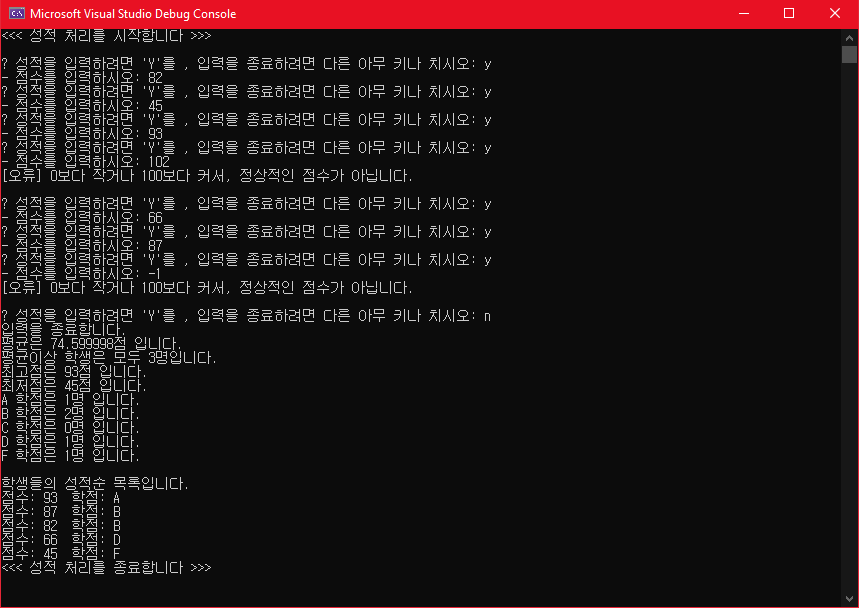
\includegraphics[width=\textwidth]{result_1.png}
            \caption{실행 결과1}
            \label{fig:result}
        \end{figure}
        
        \begin{figure}[h]
            \centering
            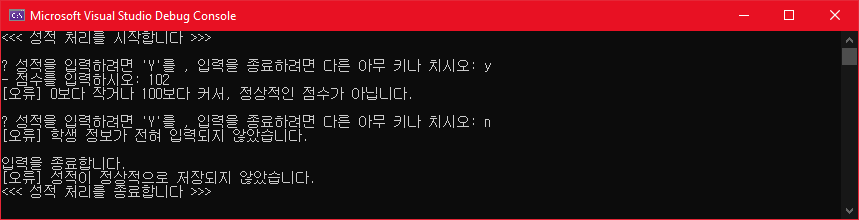
\includegraphics[width=\textwidth]{result_2.png}
            \caption{실행 결과2}
            \label{fig:result2}
        \end{figure}
        
        
        \section{입력과 출력}
            실습 자료에서 제시된 입력을 사용하였으며 출력 결과는 ~\ref{fig:result} 및 ~\ref{fig:result2} 와 같았음.
        \section{결과 분석}
            모든 입력에 대하여 정상적인 출력을 확인하였음.

    \chapter{소스코드}
        소스코드는 제출된 압축파일에 같이 동봉되어있으며 GitHub (0x00000FF/CNUCSE-Computer-Programming-III-2020-Spring) 에서도 열람할 수 있다.
\end{document}